\documentclass[stu,12pt]{apa7}
  \usepackage{times}
  \usepackage[english]{babel}
  \usepackage[utf8]{inputenc}
  \usepackage{xcolor}
  \usepackage{hyperref}
  \usepackage{enumitem}
  \usepackage{float}
  \usepackage{geometry}
  \usepackage{soul}
  \usepackage{graphicx}
  \usepackage{csquotes}
  \usepackage{endfloat}
  \usepackage{bookmark}
  \usepackage{mdframed}
  \usepackage[toc]{appendix}
  % \usepackage[backend=biber,style=apa]{biblatex}
  \usepackage{fancyhdr}
  \usepackage{mdframed}

  % Bibliography Setup
  % \addbibresource{main.bib}

  % Image Path
  \graphicspath{{res/img/}}

  % Hyperlink Setup
  \hypersetup{
    colorlinks = true,
    urlcolor = blue,
    linkcolor = blue,
    citecolor = blue
  }

  % Page and Text Layout
  \geometry{%
    a4paper,%
    top=1in,%
    bottom=1in,%
    left=1in,%
    right=1in%
  }
  \setlength{\headheight}{15pt}

  % Header
  \lhead{COM120CG1-M1D0}

  % Title Page
  \title{%
    M1D0: Student Introductions
  }
  \shorttitle{Module 1 Discussion 0}
  \author{Ashton Hellwig}
  \authorsaffiliations{Department of Mathematics, Front Range Community College}
  \course{COM115: Interpersonal Communication}
  \professor{Richard Thomas}
  \duedate{November 07, 2020 23:59:59 MDT}
  \date{\today}
  \abstract{%
    \textbf{Overview}\\%
    Welcome to COM 125—Interpersonal Communication!\\%

    The first Module 1 Discussion is titled, ``Student Icebreaker\\%
      (Introductions)''. Getting to know your classmates early on contributes to
      building a sense of community in our class.

    Read and comply with instructions 1, 2, 3, 4, and 5 appearing below.
  }

\begin{document}
  % Title Page
  \maketitle

  % Initial Post
  \section{Initial Post}
    \subsection*{Instructions}
      \begin{enumerate}
        \item Introduce yourself by name and location. Then, state your major,
          home college, career goals following graduation, why you enrolled in
          our online class (in addition to it being required), your experience
          with online classes, hobbies, favorite travel destination, favorite
          quote, how you intend to make time for completing and submitting
          classwork in accordance with due dates appearing in the Course
          Schedule, and anything else to help us get to know you better.
        \item Describe a time you communicated something via social media, text,
          or email that was completely misunderstood by the recipient.
        \item Reply to the following questions:
          \begin{itemize}
            \item Where did the problem lie, with your communication or with
              their interpretation?
            \item How did the nature of the communication (electronic versus
              face-to-face) impact understanding?
            \item What could you have done differently that would have changed
              the outcome of the communication?
            \item How have you applied what you learned from that experience to
              your communication?
          \end{itemize}
        \item Include a minimum of 100 words in your Introduction. Add a word
          count to the end of your Introduction.
        \item Finally, read the Introduction submitted by at least two
          classmates. Submit a welcome message in a reply to the Introduction
          submitted by two classmates. Remember to read and comply with the
          Class Netiquette Instructions message posted in this Discussion. You
          can do this!
      \end{enumerate}

    % Introduction
    \newpage
    \subsection{Ashton Scott Hellwig's Personal Introduction}
      Hello, everyone! My name is Ashton Scott Hellwig, but closer friends refer
        to me using my initials: Ash. I live in Lafayette, Colorado and my major
        is declared as ``Associate of Science: Mathematics for Transfer''. My
        Home College is Front Range Community College, mainly in the online
        medium for the last two years with only one in-person class I took in
        2018. I prefer enrolling in online classes because it allows me more
        freedom to continue working my normal full-time hours and get school
        work complete without having to be physically present in a classroom.
        Because of my experience working in IT remoteley before switching to
        the industry I am in currently, online class was not too large an
        adjustment for me. One of my favorite hobbies is where I am currently
        working with various protection dog training schools as an protection
        dog training apprentice and agitator.

        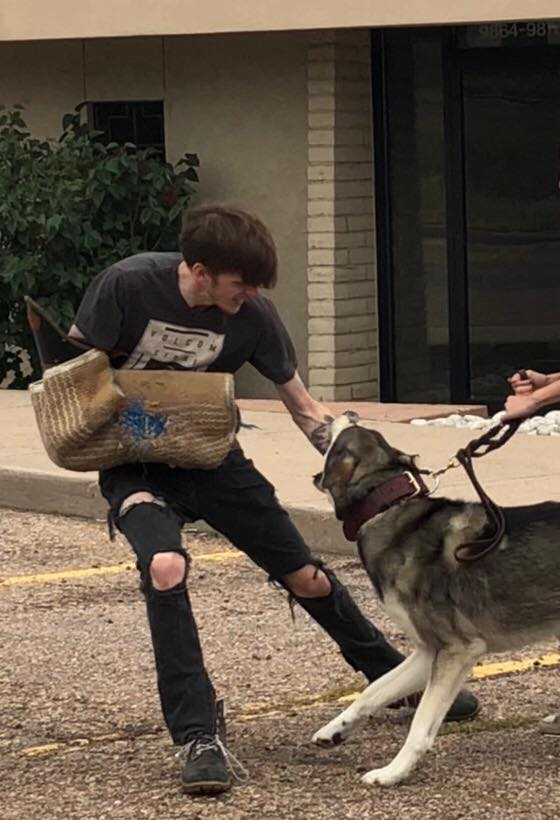
\includegraphics[height=100px,width=100px]{KojackBiteWork1}

        I plan on making time to complete this class whenever I can fit it in,
        which is pretty easy for me to do throughout the day as well as after
        work. I recently purchased a laptop for this specific purpose, so I am
        able to complete tasks throughout my work day. I am an inventory manager
        at a marijuana dispensary in Denver, and even though the cannabis
        retail industry is even more hectic during the essential-business
        designation than ever before I will still have significant time
        available to complete assignments as I have consistent schedule where I
        am out of work by 6:00PM every day. I don't really travel so much with
        the exception of to Atlanta and Los Angeles. I was born in Kansas, then
        lived in St.\ Louis for 2 years, then in Birmingham for 3 years, and
        finally spent most of my childhood until my sophomore year of High
        School in Atlanta. I moved to Colorado in 2013 and when the rest of my
        family left for Los Angeles in 2016 I decided to stay here. With my
        degree, I want to go into veterinary bioinformatics research but my
        ultimate goal is to own my own licensed MIP here in Colorado foucusing
        on the solventless extraction of rare cannabinoids. Progress is being
        made on this day-by-day!

      One time I can remember where an email was misunderstood by the recipient
        was towards the beginning of the pandemic entering our daily lives at
        the previous dispensary I worked as compliance assurance officer. I had
        sent an email to the head of our legal department and the general
        manager for the store I was located at detailing my reasons for not
        wanting to bring customers back inside and to continue the curbside
        pickup process as long as possible citing concerns from many employees
        which fell on deaf ears and they believed I was not ``towing the line''
        as I should have been and that my tone was too aggressive. This led them
        to say ``Either get behind our decisions, good or bad, or it is a very
        good time to collect unemployment right now''. I believe the
        miscommunication lied within the fact that without being able to
        effectively deliver tone through email, along with using ``urgent''.
        sounding speech, this could have come off as rude or aggressive to them.
        I avoid this nowadays by utilizing telephone or face-to-face to discuss
        important matters rather than attempting an urgent sounding email.



    % Replies
    % %! TEX root='..\main.tex'

\part{}

\end{document}
